\chapter{提案手法}
\section{センサノードグループ化}
\subsection{想定する環境}
想定するセンサデバイスは,異種無線の通信機能を持つモジュールを搭載している.想定するLoRaWAN ネットワークは,3つのコンポーネントからなり,センサノード・ゲートウェイ(GW: Gateway)・ネットワーク制御を行うネットワークサーバ(NS: Network Server)から構成されたスター型トポロジである.LoRaWANは,デバイスが安価であり利用において免許を必要としないため,都市部のような密集地域では,センサノードが隣接している可能性が考えられる.従って,想定する環境は,異種無線によるグループ化の適応機会が望める都市部のようなセンサノードが密集した地域である.
\subsection{センサノードグループ化とグループ再構成の必要性}
提案手法では,消費電力の削減,及びバッテリ残量の平準化の面で消費電力の効率化を図る.近傍の通信メッセージを代表にて集約しGWノードまでの長距離伝送の利用を減らすことで省電力化を狙う.管理コストを削減するためバッテリ交換のタイミングは同時にまとめて行える方が良く,センサノード間でのバッテリ残量の平準化の実現が望ましい.省電力化のため,異種無線(LoRaWAN,BLE)を用いて,グループ化により近傍ノード(GM: Group Member)のデータを代表ノード(GL: Group Leader)が集約する(図1).バッテリ残量平準化のため,グループの再構成を行う.起動時やトポロジ変化後などグループが定義されていない展開時の設定手法と稼働中に行われる再構成手法を以下に説明する.
%---
\section{センサノードグループ化のアプローチ}
\subsection{トポロジ}
グループは,ある数のセンサノードから構成される.グループ化のトポロジは,グループ内ではGMノードにGLノードが接続しGLノードとGWノードが接続するスター型トポロジとなる.

\begin{figure}[]
    \begin{center}
    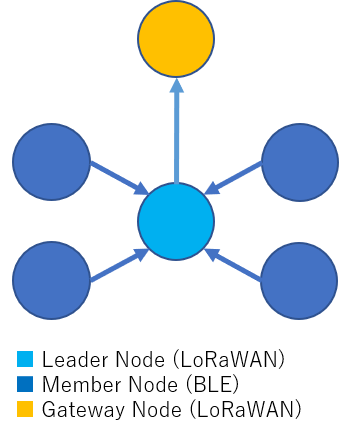
\includegraphics[width=5cm]{figures/グループ化のトポロジ.png}
    \caption{グループ化のトポロジ}
    \label{fig:group_topology}
    \end{center}
\end{figure}
\subsection{センサネットワーク展開時のグループ化}
センサネットワークが展開される初回起動時にグループを作成する手法を述べる.GWノードがセンサノードのトポロジを把握するため,各ノードが周囲のノード情報を探索する.下記にシーケンス図\ref{fig:group_on_activation}を示す.

\begin{enumerate}
    \item グループを構築するに当たり,GWノードに現在のWSNトポロジを通知する必要がある.そのため,センサノード起動時に,BLEにて自身の情報を発信し,同時に周囲のセンサノード情報を収集する.近傍センサノードのリストを作成した後,GWノードへ送信する.
    \item センサノードはリスト送信後,GWノードからグループ構成の通知が来るまでLoRaWANにて通信を行う.
    \item GWノードがセンサノード情報を集約した後,センサノードの固有ID,及び個々の信号強度を用いて重複ノードのないグループを作成しグループごとに1つGLノードを選出する.センサノードがLoRaWANにて次に接続した場合,Downlinkでグループ構成を通知しシーケンスは終了する.
\end{enumerate}

\begin{figure}[]
    \begin{center}
    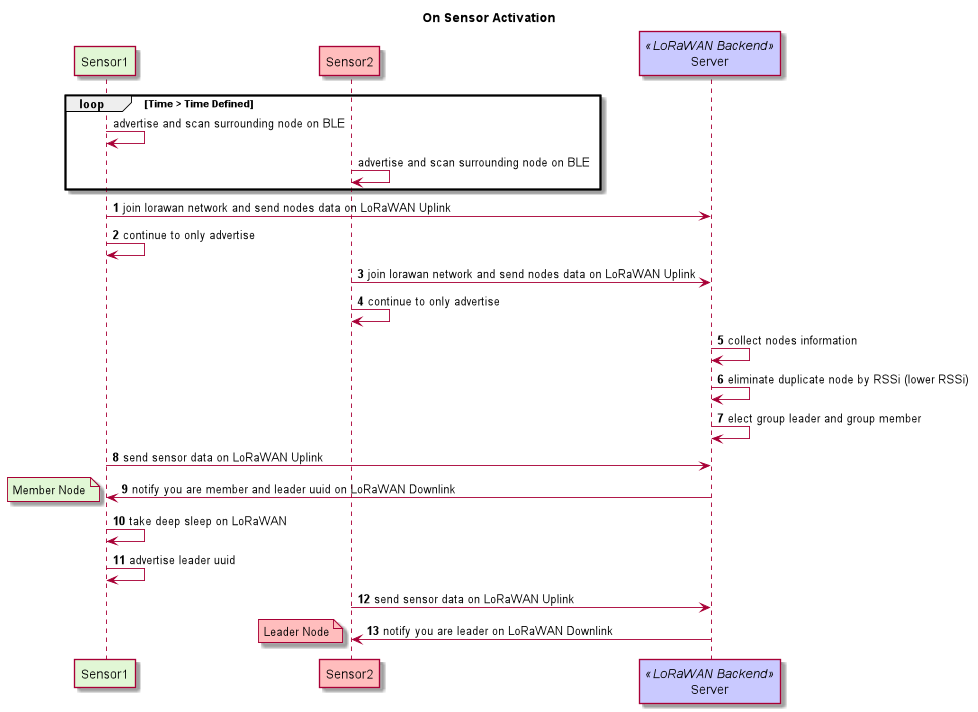
\includegraphics[width=14cm]{figures/グループ化_センサ起動時.png}
    \caption{グループ化の通信方式}
    \label{fig:group_on_activation}
    \end{center}
\end{figure}
\subsection{平常時のグループ化の通信}
平常時のグループの通信フローを述べる.通信方式は,グループ内の通信にBLE,GLノードとGWノードの通信にLoRaWANを用いる.グループ内の通信は,インターバルが設けられ同期的に通信を行う.下記にシーケンス図\ref{fig:default_data_flow}を示す.

\begin{enumerate}
    \item GMノードはGLノードとの接続要求のため,Advを開始する.
    \item GLノードはGMノードとの接続確立のため,BLEにてScanを開始する.
    \item GLノードは接続確立後,GMノードからセンサデータを集約しGWへ送信する.
    \item WSNに新たなノードが参加した際にグループに所属するため,GLは自身のサービスUUIDを載せAdvを開始する.
\end{enumerate}

\begin{figure}[]
    \begin{center}
    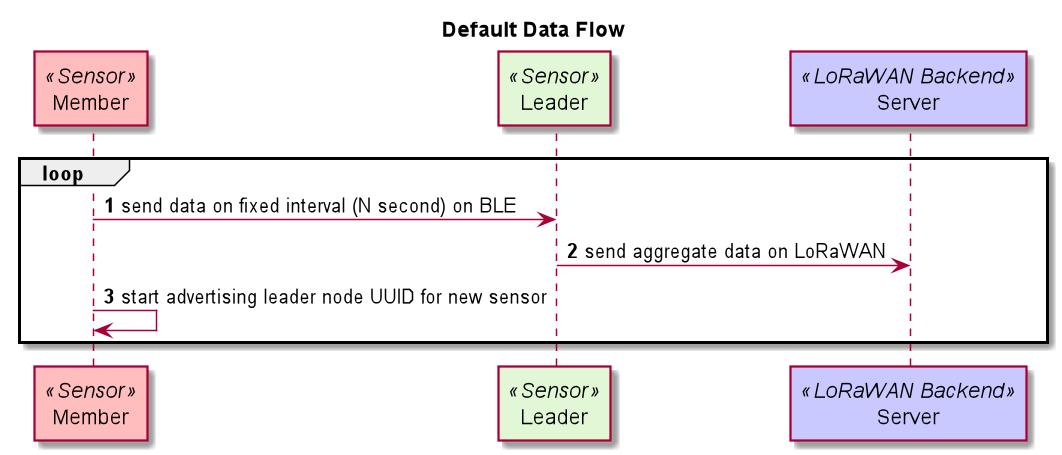
\includegraphics[width=13cm]{figures/グループ化の通信方式.png}
    \caption{グループ化の通信方式}
    \label{fig:default_data_flow}
    \end{center}
\end{figure}
\subsection{センサノードの参加・離脱時の振る舞い}
いくつかのセンサノードが,グループへ参加・離脱する際の手法を述べる.\\ \\
前者について下記にシーケンス図\ref{fig:group_on_join}を示す.

\begin{enumerate}
    \item 新規センサノードがグループに参加するため,参加するグループを決定する必要がある.GLノードはデータ集約時以外は,Adv Packetに自身のBLEサービスUUIDを載せAdvを行う.
    \item 新規センサノードは,起動時にBLEスキャンを実行し周囲に参加可能なグループがあるか探索する.
    \item 発見した場合は,そのグループに参加し,そうでない場合はLoRaWANで直接センサデータを送信する.
\end{enumerate}

後者について,下記にシーケンス図\ref{fig:group_on_leave}を示す.

\begin{enumerate}
    \item ノードが故障や電池切れで離脱する場合は,NSがデバイスを管理しているので,N回通信が来なかった場合に,グループリストからセンサノードを取り除く.
    \item GLノードの次回通信時に,更新したグループリストを通知する.
\end{enumerate}

\begin{figure}[]
    \begin{center}
    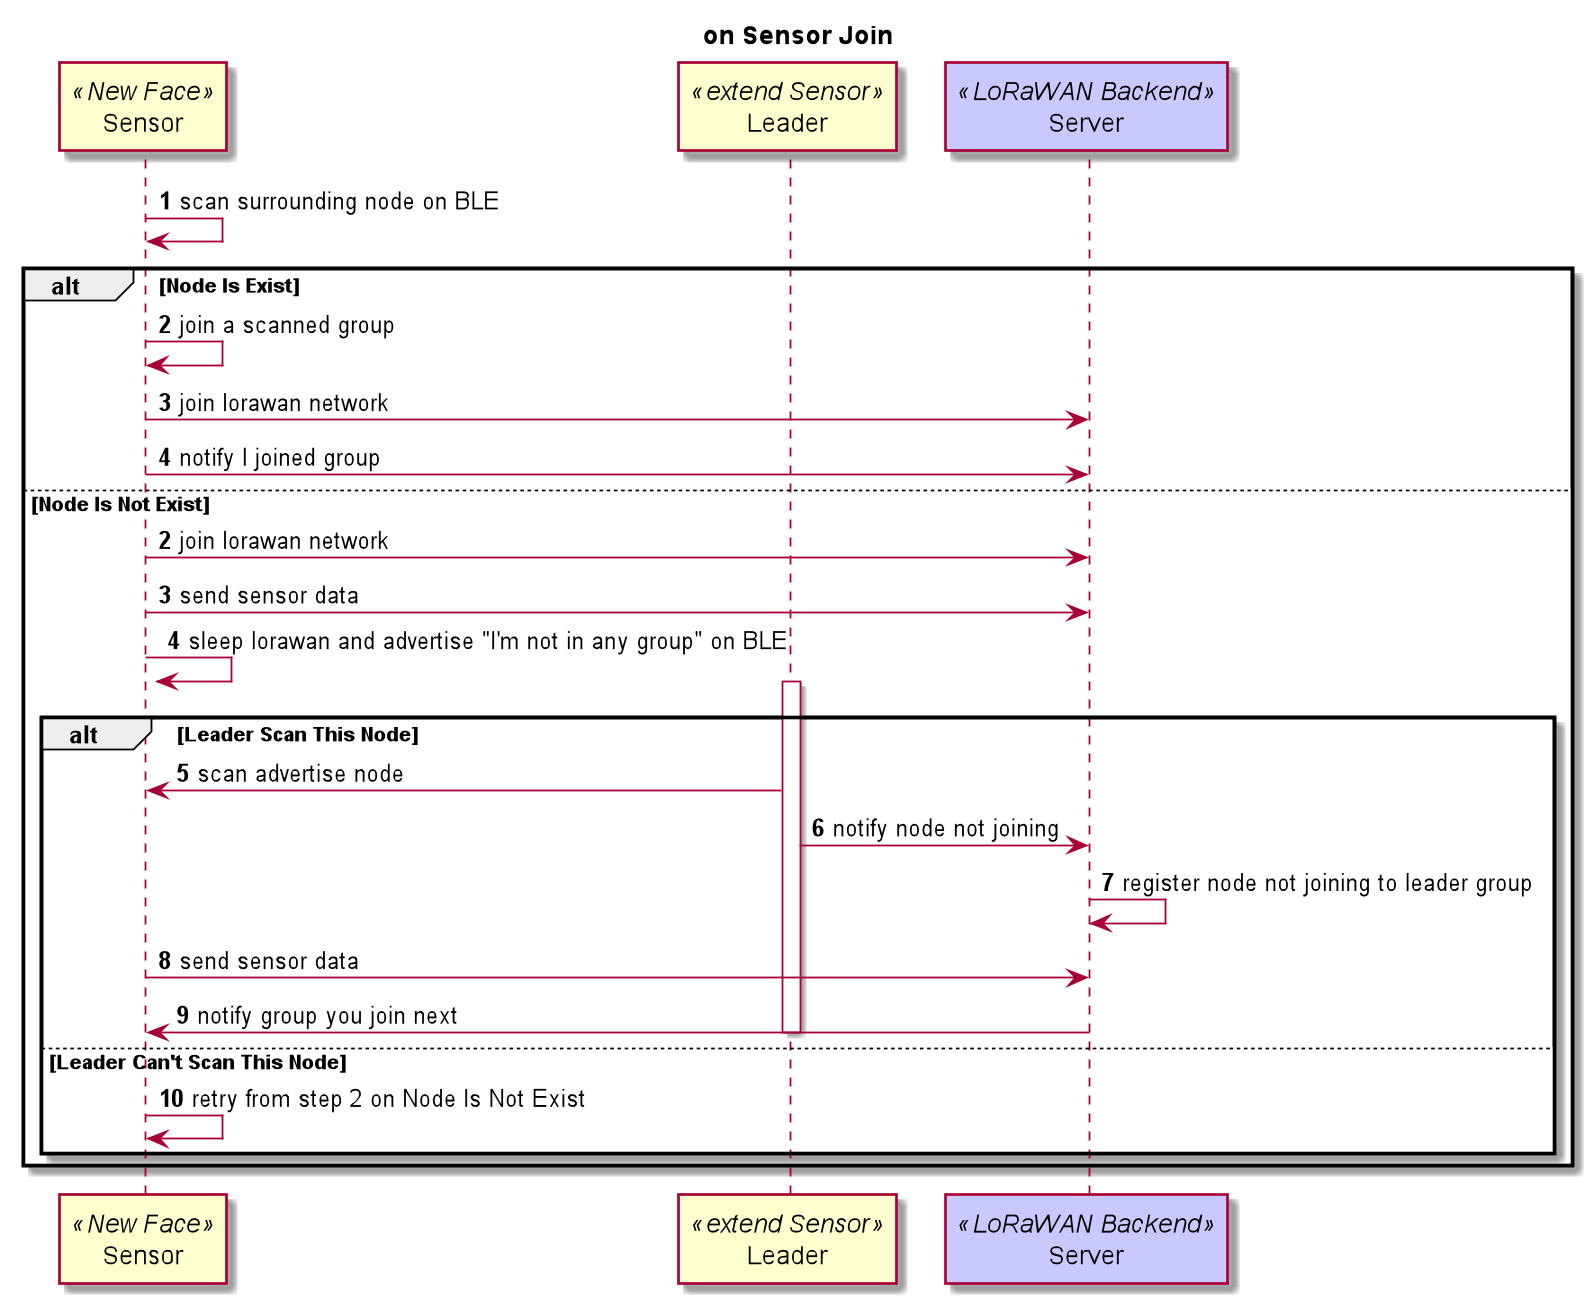
\includegraphics[width=14cm]{figures/グループ化_ネットワーク参加時.png}
    \caption{ネットワーク参加時の振る舞い}
    \label{fig:group_on_join}
    \end{center}
\end{figure}


\begin{figure}[]
    \begin{center}
    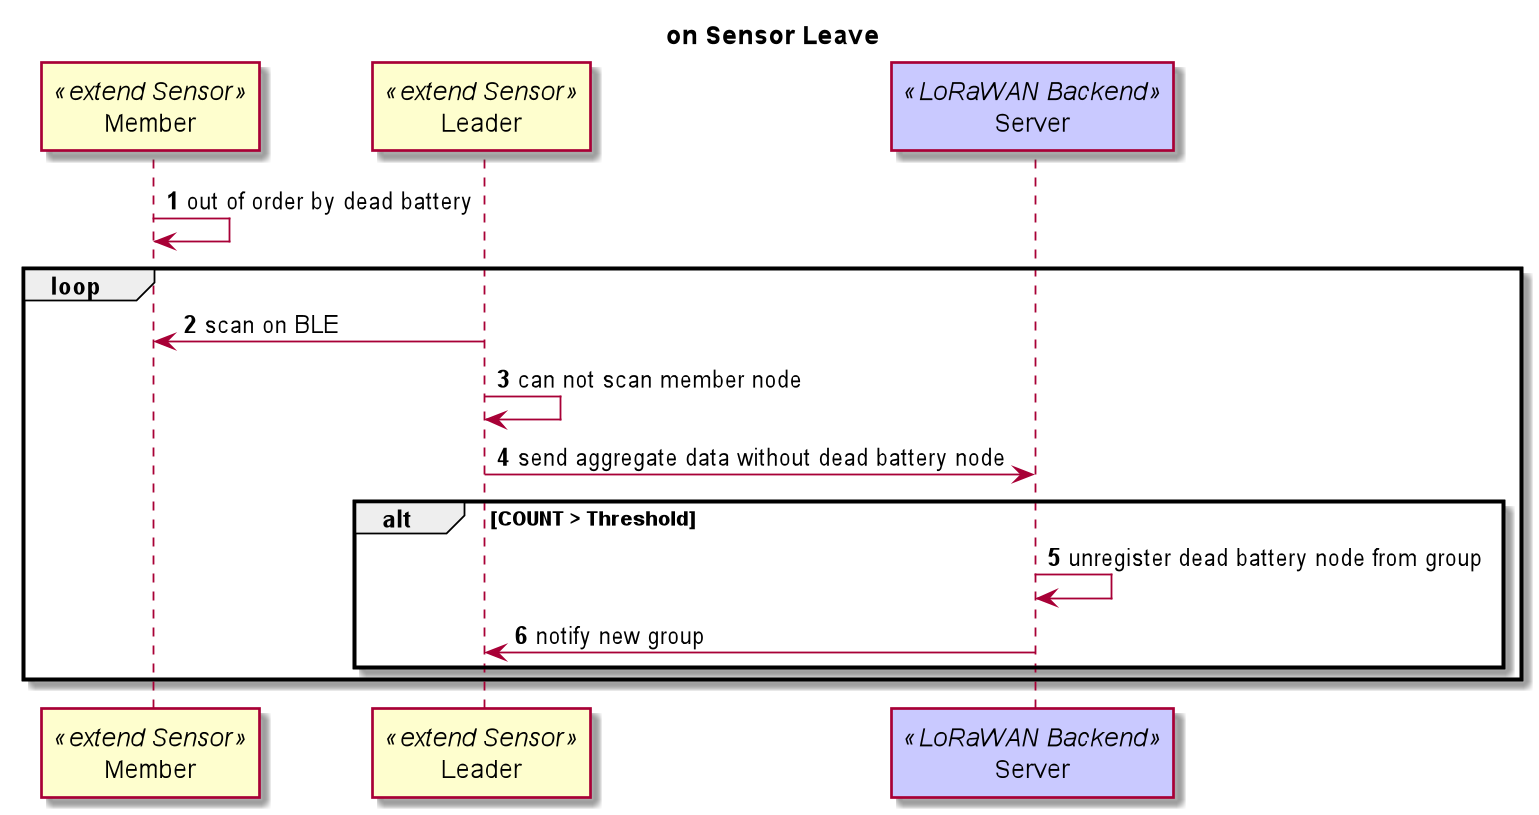
\includegraphics[width=14cm]{figures/グループ化_ネットワーク離脱時.png}
    \caption{ネットワーク離脱時の振る舞い}
    \label{fig:group_on_leave}
    \end{center}
\end{figure}
%---
\section{センサノードグループ再構成のアプローチ}
\subsection{自律型再グループ化}
グループ内で,GLを交代し電力の平準化を図る自律型グループ化\ref{fig:group_reconstruction_independently}について述べる.全センサノードは,LoRaWAN及びBLEでの通信回数を保持している.(電力式)により,総消費電力量を見積もり可能となる.GLノードはGMノード通信時に総消費電力量を取得する.GLはGMノードの消費電力量を基に,最も消費が少ないGMノードを次のGLとして選出したのちGMへ通知する.後にデータを集約しGWへ送信する.これにより,グループ内でのセンサノードの消費電力を平準化が見込める.

\begin{figure}[]
    \begin{center}
    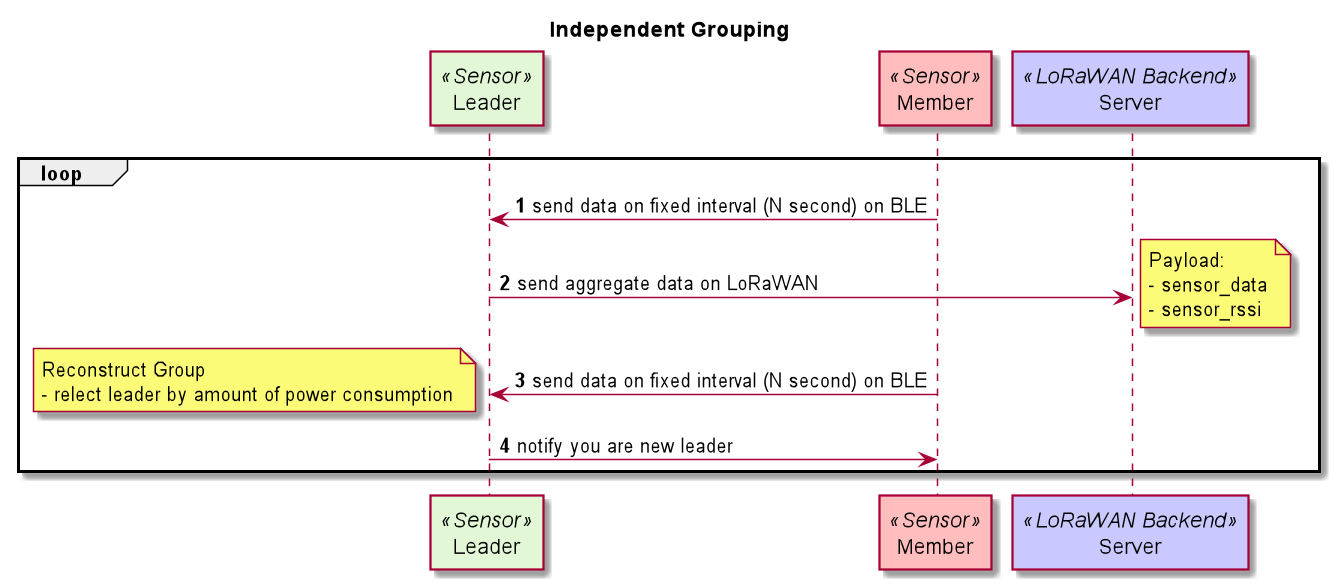
\includegraphics[width=14cm]{figures/グループ化_自律的.png}
    \caption{自律型再グループ化}
    \label{fig:group_reconstruction_independently}
    \end{center}
\end{figure}
\subsection{集中型再グループ化}
グループの構成を変更し,WSN全体での電力の平準化を図る集中型グループ化について述べる.WSN内にセンサノードが追加されていくと,初期に構築したグループでは最適でない場合が考えられる.そのため,GWノードはセンサノードから取得したデータ(デバイス固有ID・信号強度)を用いて最適なグループを再構成する.下記にシーケンス\ref{fig:group_reconstruction_concentrately}を示す.

\begin{enumerate}
    \item GMノードは,定常時と同様センサデータをGLノードへ送信する.
    \item GWノードは,データとして各センサノードの異種無線利用回数から消費電力量を算出する.
    \item GWノードは,センサデータの信号強度(RSSi),消費電力量からグループ間でのノード移動やGLの交代などの組み合わせを検討し,グループを再構成する.
    \item GWノードは,センサノードのダウンリンク時に再構成したグループを通知する.
\end{enumerate}

これにより,センサネットワーク全体の消費電力を平準化でき,センサ交換機会の削減が見込める.

\begin{figure}[]
    \begin{center}
    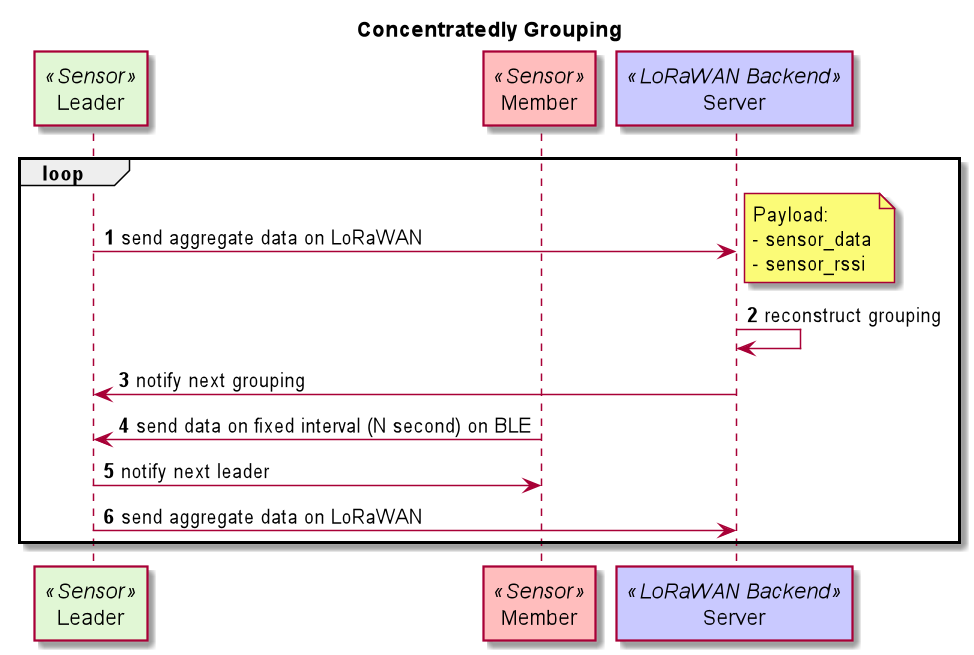
\includegraphics[width=14cm]{figures/グループ化_集中的.png}
    \caption{集中型グループ化}
    \label{fig:group_reconstruction_concentrately}
    \end{center}
\end{figure}